\begin{Exercise}[title=($*$) Fibre de verre]
  La fibre de verre de longueur $l$ et de diamètre $d$ et de masse volumique
  $\rho=$\SI{2500}{\kg\per\m\cubed} est encastrée horizontalement dans une paroi
  immobile. Au repos, la fibre est horizontale (on néglige son poids). Quand on
  applique une force verticale $F$ (on supposera que la force $F$ reste
  verticale tout au long de l’expérience) à l’extrémité libre de la fibre,
  celle-ci est déformée. L’extrémité est déplacée verticalement d’une distance
  $Y$ que l'on appelle la flèche.
  % \begin{figure}[h!]
  \begin{center}
    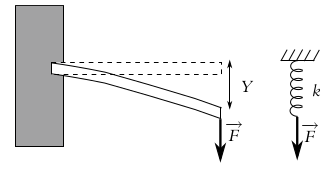
\includegraphics[scale=0.5]{./fig/fibre_ressort.png}
  \end{center}
  % \end{figure}
  La flèche Y est donnée par la relation suivante (on notera la présence du
  facteur numérique 7, sans dimension, qui est en fait une valeur approchée pour
  plus de simplicité) :$Y=\frac{7l^3F}{Ed^4}$ où E est appelé module d’\textsc{Young} du
  verre. Pour les applications numériques on prendra pour le module d’\textsc{Young}
  $E = 7.10^{10} S.I.$
  \Question Quelle est l’unité S.I. du module d’\textsc{Young} E ?
  \Question En considérant uniquement la force F, montrer que l’on peut
  modéliser la fibre de verre par un ressort de longueur à vide nulle et de
  constante de raideur k dont on donnera l’expression analytique en fonction de
  $E$, $d$ et $l$
  \Question Calculer numériquement k pour une fibre de longueur
  \gdr{l}{7}{mm} et de diamètre \gdr{d}{10}{\um}
  \Question Démontrer l’expression de l’énergie potentielle élastique d’un ressort de longueur à
  vide nulle, de constante de raideur k, lorsque sa longueur est $l$. En
  reprenant l’analogie du ressort, quelle est alors l’énergie potentielle
  élastique de la fibre de verre lorsque la flèche vaut Y?
  \Question On a tous fait l’expérience suivante : faire vibrer une règle ou une tige lorsque une de
  ses extrémités est bloquée. On cherche ici à trouver les grandeurs pertinentes
  qui fixent la fréquence des vibrations. L’extrémité de la tige vaut Y (t) à
  l’instant t. On admet que lors des vibrations de la fibre, l’énergie cinétique
  de la fibre de verre est donnée par l’expression:
  $E_c = \rho l d^2 \left(\dd{Y}{t}\right)^2$
  \Question Écrire l’expression de l’énergie mécanique de la fibre en négligeant
  l’énergie potentielle de pesanteur.
  \Question Justifier que l’énergie mécanique se conserve au cours du
  temps. En déduire l’équation différentielle qui régit les vibrations de la
  fibre.
  \Question Quelle est l’expression de la fréquence propre de vibration
  d’une tige de verre de module d’\textsc{Young} $E$, de longueur $l$ et de diamètre $d$.
  \Question Calculer numériquement la fréquence des vibrations d’une fibre de
  verre de longueur \gdr{l}{7}{mm} et de diamètre \gdr{d}{10}{\um}
\end{Exercise}
\begin{Answer}
	\Question E est en Pascal (Pression)
	\Question On considère l’extrémité de la fibre comme un point matériel. Les
    deux forces s’exerçant sur ce point sont F et la tension T du ressort
    équivalent cherché qui est vers le haut. L’équilibre de l’extrémité donne la
    relation entre les forces: $T= -F =- \underbrace{\frac{Ed^4}{7l^3}}_{k}Y $

	\Question k = $2,9.10^{-4}$ N/m
	\Question  on a $dE_p= -\delta W= -T dl = -kldl  \Rightarrow E_p= \frac{1}{2}kl^2 + \underbrace{C}_{=0}$
	d'ou : $E_p = \frac{1}{2}\frac{Ed^4}{7l^3}Y^2$
	\Question $E_m=\frac{Ed^4}{14l^3}Y^2+\rho l d^2 \left(\dd{Y}{t}\right)^2$
	\Question Force conservatives seule présente.
	$\dd{Em}{t}=0 \Rightarrow \dot{Y}\left(\frac{Ed^4}{7l^3}Y+2\rho ld^2 \ddot{Y}\right) =0$
	$\ddot{Y}+\frac{Ed^4}{14\rho l^4}Y=0$
	\Question $\omega_0= \sqrt{\frac{Ed^2}{14\rho l^4}} $
	\Question $f_0=45,9Hz$
\end{Answer}
